In finite element modeling, a finer mesh typically results in a more accurate solution. However, as a mesh is made finer, the computation time increases. To get a mesh that satisfactorily balances accuracy and computing resources a mesh convergence study was performed

In this scope, the breast and muscle geometries was meshed with different mesh sizes; the minimal elements sizes was set to $7mm$ and the maximal element size was varied between $\lbrace 7mm$,  $10 mm$, $13mm$, $15mm$, $17mm$, $20mm\rbrace$. The compression paddles geometries were meshed with a constant element size of $1mm$. The number of elements obtained for each mesh size is given in Table  \ref{nbElementsvsmeshsize}. For the mesh size equal to 17 mm, a higher number of elements is obtained then compared to the  mesh size of 15mm. As  mesh size is defined by the maximal and minimal elements size, a higher number of \textit{small} elements was needed to cover the areas smaller than the \textit{large} elements. In such meshes the elements density is normally concentrated on the geometry's corners or narrow spaces which, in our case, dose not coincide with the region of interest.  

\begin{table}[!h]
\begin{tabular}{|c|c|c|c|c|c|c|}
\hline
Mesh size & 20mm & 17mm & 15mm & 13mm & 10mm & 7mm \\
\hline
Nb. of elements & 8367 & 10897 & 8099 & 10751 & 18453 & 65785 \\
\hline
\end{tabular}
\caption{Number of elements obtained for each mesh size.}
\label{nbElementsvsmeshsize}
\end{table} 

As the model was conceived to model breast deformation under compression, an equivalent simulation was performed to estimate the optimal mesh size. Starting from the breast supine geometry, the gravity was applied in the posterio-anterior direction. Then, the right breast was compressed between the compression paddles (Figure \ref{fig:meshconvergence}). The strain distribution over the breast volume as well as the compression force for each mesh size are given in the Figure \ref{fig:meshconvergence}. 

\begin{figure}[!h]
\centering
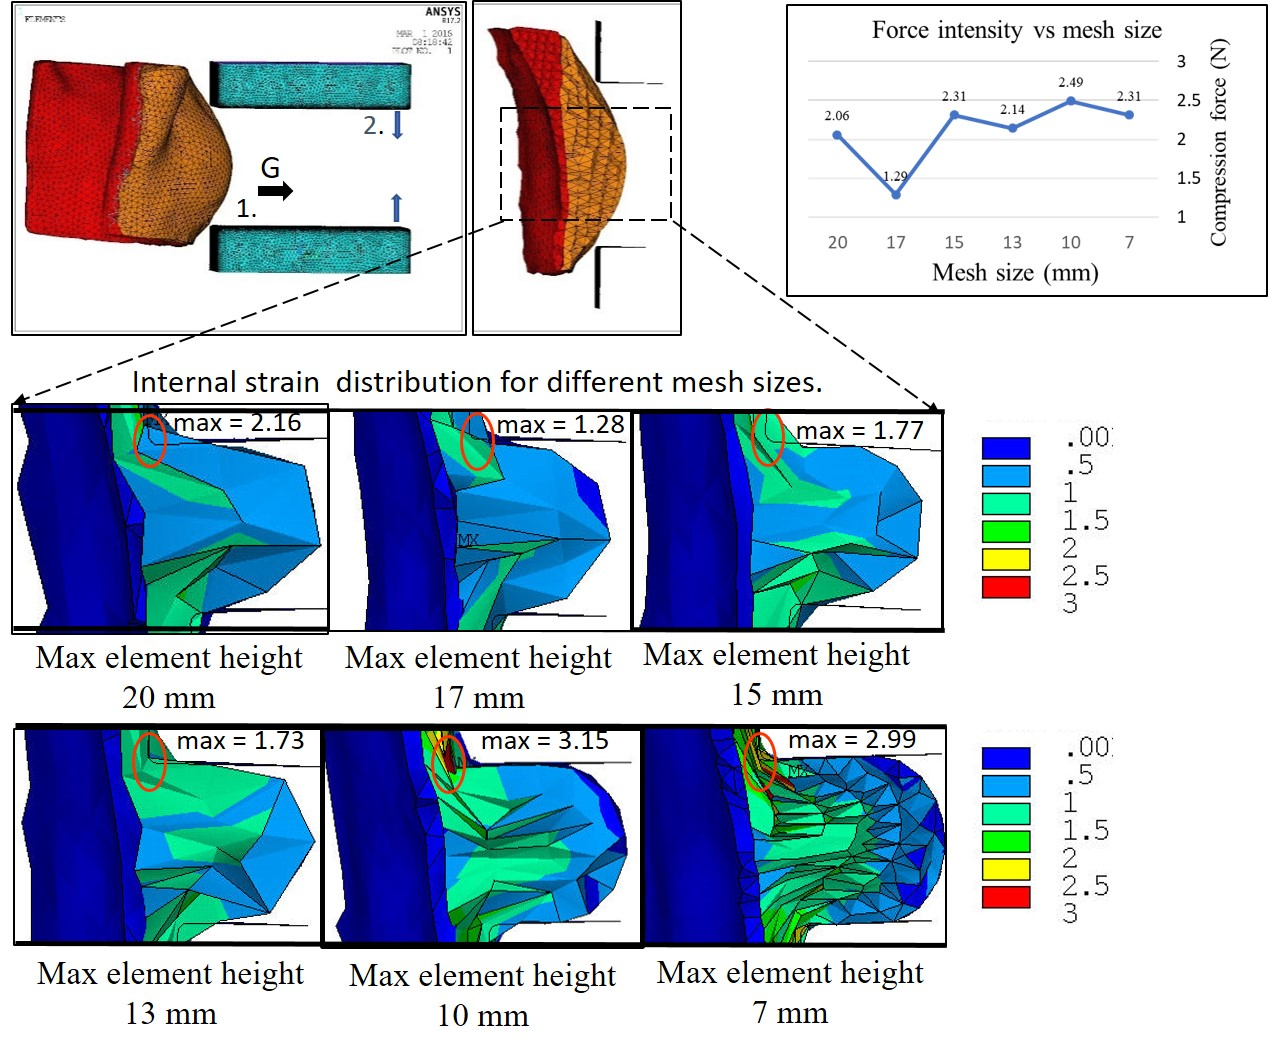
\includegraphics[width=\textwidth,keepaspectratio]{figures/meshConvergence.jpg} 
\caption{Internal strain distribution in function of the elements size. }\label{fig:meshconvergence}
\end{figure}

One can see, that the force intensity converges from a mesh size equal to $15mm$, however the strain distribution over the breast volume have still a poor estimation when compared to the strain distribution obtained with a mesh size equal to 7mm. The visual analysis of the strain distribution and amount of penetration at the surface contact  shows that stating from a mesh size equal to 10mm the results are well enough estimated. 